%============================== Setting teh Document=============================================

\documentclass[aspectratio=169]{beamer}
\usepackage[english]{babel} 
\usepackage[utf8]{inputenc} 
\usepackage[T1]{fontenc}
\usepackage{graphicx}
\usepackage{xcolor}
\usetheme{AnnArbor}
\usepackage{multicol}
\usepackage[pscoord]{eso-pic}
\usepackage{tikz}
%==========================Set the foot line========================================================

\setbeamercolor*{author in head/foot}{parent=palette tertiary}
\setbeamercolor*{title in head/foot}{parent=palette primary}
\setbeamercolor*{date in head/foot}{parent=palette primary}

\defbeamertemplate*{footline}{}
{
	\leavevmode
	\hbox{%
		\begin{beamercolorbox}[wd=.25\paperwidth,ht=2.25ex,dp=1ex,center]{author in head/foot}%
			% << Add Telephone Number >>
			\usebeamerfont{author in head/foot}\centering{}
		\end{beamercolorbox}%
	
		\begin{beamercolorbox}[wd=.25\paperwidth,ht=2.25ex,dp=1ex,center]{title in head/foot}
			% << Add Mobile Number >>
			\usebeamerfont{title in head/foot}\centering{Numero di Cellulare}
		\end{beamercolorbox}%
	
	        \begin{beamercolorbox}[wd=.25\paperwidth,ht=2.25ex,dp=1ex,center]{author in head/foot}%
	        	% << Sostituisci i miei indirizzi mail con i tuoi >>
	   	 		\usebeamerfont{author in head/foot}\centering{\href{mailto:f.rombaldoni@campus.uniurb.it}{f.rombaldoni@campus.uniurb.it}}
    	    \end{beamercolorbox}%

		\begin{beamercolorbox}[wd=.25\paperwidth,ht=2.25ex,dp=1ex,center]{date in head/foot}%
			% << Replace with your name >>
			\usebeamerfont{date in head/foot}\centering{Luca Brici}\hspace*{2em}
		\end{beamercolorbox}}%
}
\AddToShipoutPictureFG{
	\put(\LenToUnit{.884\paperwidth},
	\LenToUnit{.25\paperheight})
	{\vtop{{\null}
	\makebox{\begin{tikzpicture}
	% << Qui è dove puoi mettere la tua immagine profilo>>
	\clip (0,0) circle (6mm) node {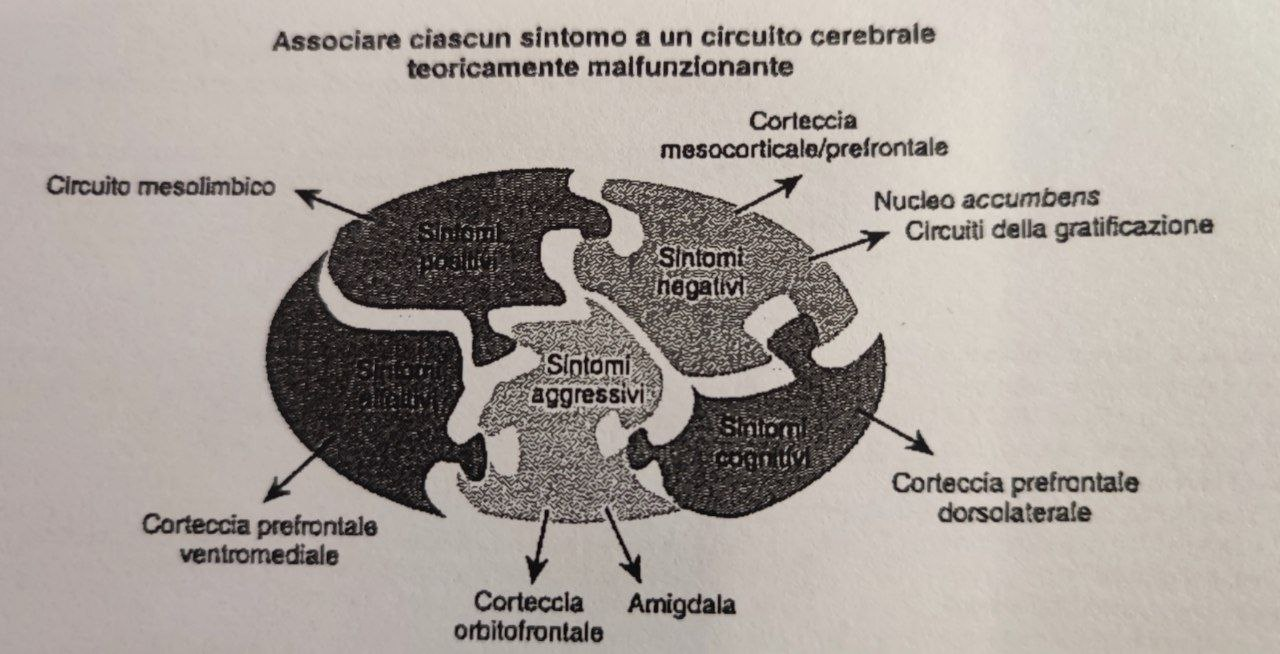
\includegraphics[width=22mm]{Images/Immagine_profilo.jpg}};
	\end{tikzpicture}}}}} 

%===========================================Document starting===============================================
\begin{document}

% << First line of text to change >>
\section{La pratica del prestare attenzione, trovarla per scegliere dove dirigerla.}
\setbeamertemplate{navigation symbols}{}
% << Change the title >>
\begin{frame}[t]{\textbf{CORSO Di MINDFULNESS}}
	
	\mbox{
	\colorbox{gray!20}{\begin{minipage}[t][0.8\textheight][t]
			{\dimexpr0.78\textwidth-2\fboxsep-2\fboxrule-5pt\relax}
			\raggedright
			\small
			Quando si parla di meditazione o di mindfulness, ci si immagina il monaco che medita nel tempio buddhista o comunque qualcosa di stereotipato e lontano dalla vita quotidiana. In realtà la mindfulness è qualcosa di molto più semplice e alla portata di tutti, in quanto non è altro che un particolare modo di prestare attenzione a ogni cosa della nostra vita.\\
			\vspace*{1.5mm}
			Spesso passiamo la nostra vita in uno stato di mancanza di consapevolezza, che può comportare tutta una serie di conseguenze negative.\\
			\vspace*{1.5mm}
			La mindfulness ci permette di:
			\vspace*{1.5mm}
			\begin{itemize}
				\item Essere più consapevoli, e quindi vivere davvero ogni momento.
				\item Riuscire a ridurre stress e ansia, abbandonando i giudizi che abbiamo su noi stessi e gli altri.
				\item Riuscire a sostituire i comportamenti automatici disfunzionali con comportamenti consapevoli e	funzionali.
			\end{itemize}
	\end{minipage}}

\colorbox{gray!20}{\begin{minipage}[t][0.8\textheight][t]
		{\dimexpr0.22\textwidth-2\fboxsep-2\fboxrule-5pt\relax}
		% << Aggiorna qui il contatto di  WhatsApp>>
		\centering{\textbf{Cercami su WhatsApp}}
			\begin{figure}
			\centering
			% << Qui metti la tua immagine del qr-code di WhatsApp >>
			
\includegraphics[width=0.5\textwidth]{Images/WhatsApp-QR-code.png}
		\end{figure}
			% << Aggiorna qui il contatto di Telegram>>
		\centering{\textbf{Cercami su Telegram}}
	\begin{figure}
		\centering
		% << Qui metti la tua immagine del qr-code di Telegram>>
		
\includegraphics[width=0.5\textwidth]{Images/Telegram-QR-code.png}
	\end{figure}
	\end{minipage}}
}

\end{frame}

\end{document}
